\documentclass{article}

% if you need to pass options to natbib, use, e.g.:
% \PassOptionsToPackage{numbers, compress}{natbib}
% before loading nips_2017
%
% to avoid loading the natbib package, add option nonatbib:
% \usepackage[nonatbib]{nips_2017}

\usepackage[final]{nips_2017}


\usepackage[utf8]{inputenc} % allow utf-8 input
\usepackage[T1]{fontenc}    % use 8-bit T1 fonts
\usepackage{hyperref}       % hyperlinks
\usepackage{url}            % simple URL typesetting
\usepackage{booktabs}       % professional-quality tables
\usepackage{amsfonts}       % blackboard math symbols
\usepackage{nicefrac}       % compact symbols for 1/2, etc.
\usepackage{microtype}      % microtypography
\usepackage{graphicx}
% Choose a title for your submission
\title{Your title here}


\author{Student 1 \qquad Student 2 \qquad Sandar Felicity Lim}
\graphicspath{ {fig/} }
\begin{document}
% \nipsfinalcopy is no longer used

\maketitle

% We do not requrire you to write an abstract. Still, if you feel like it, please do so.
%\begin{abstract}
%\end{abstract}

Feel free to add more sections but those listed here are strongly recommended.
\section{Introduction}
You can keep this short. Ideally you introduce the task already in a way that highlights the difficulties  your method will tackle.

\section{Methodology}
\subsection{Generating wrong endings}
Wrong endings were generated for each story to better train our classifier. Naive way would be to randomize the correct endings of each story. However, doing so would obviously change the main charecter or main point of the story. Therefore, we needed to generate endings that are wrong but still preserves narrative structure. Negation of the fifth sentence was a promising way to achieve that end. i.e. The resulting sentence would be contain at least one of the charecters of the story. The resulting sentence would still be generally realisitic, except that it would not create a meaningful story as an addition to the previous four sentences.

Negation can be challenging when we have more complex sentence structures. For example,
Emma...


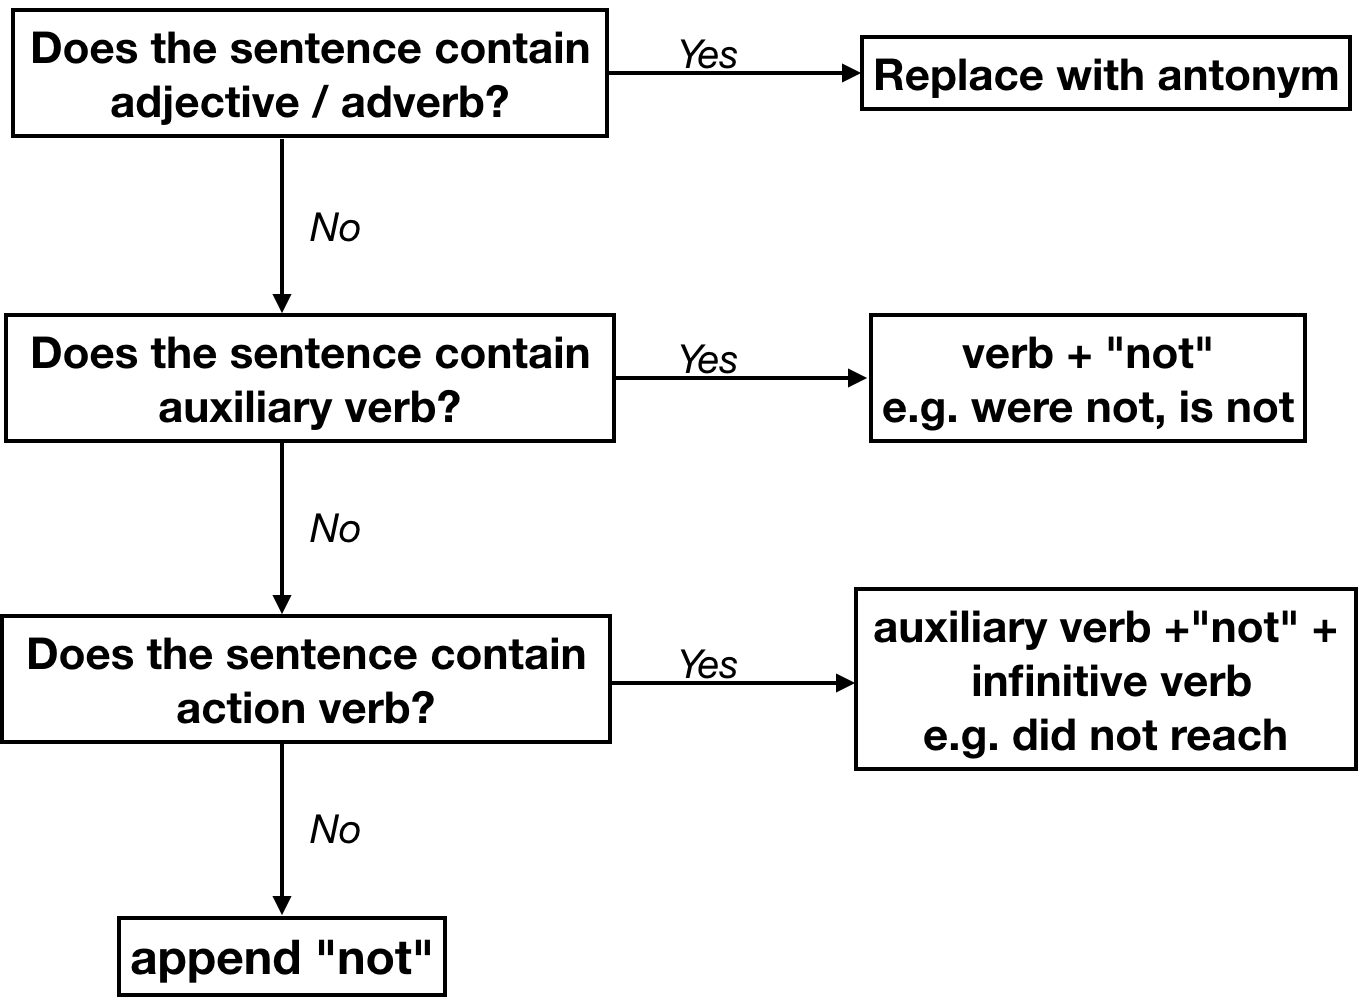
\includegraphics[width=0.9 \linewidth]{wrong.PNG}


strange: ,Tom hit a watery oily patch.,He spun out of control and hit a tree.,Tom was paralyzed from the neck down., Tom was not paralyzed from the neck down .,Tom was not paralyzed from the neck down .,Tom was paralyzed from the neck down.,Tom was not paralyzed from the neck down .,1

Too Much Candy,Laura found a jar of candy in her mom's kitchen.,Laura ate all of the candy.,She got really sick.,Laura's mom discovered why Laura was sick.,Her mom felt bad for her so she didn't punish her for eating it all., Her mom felt good for her so she did n't punish her for eating it all .,Her mom felt good for her so she did n't punish her for eating it all .,Her mom felt bad for her so she didn't punish her for eating it all.,Her mom felt good for her so she did n't punish her for eating it all .,1

did not work:
Once he grew up he realized he wanted to do other things.,His dad was very angry.,Their relationship got bad and they no longer talked., Their relationship got good and they no longer talked .,Their relationship got good and they no longer talked .,Their relationship got good and they no longer talked .,Their relationship got bad and they no longer talked.,2

25438bdc-2b79-4f57-ab33-8406018619e9,Dress,I was shopping for a dress for my daughter.,I wanted to find something that fit her personality.,"She is very creative, so I looked for something unusual.",I found a dress that was red and had pretend paint splatters.,"I went home happy, having found the perfect dress."," I went home happy , having found the imperfect dress .","I went home happy , having found the imperfect dress .","I went home happy, having found the perfect dress.","I went home happy , having found the imperfect dress .",1

works:
0440d713-98c7-494a-9021-98750467a5f9,Tumbling Down,Tim was hiking up a mountain with friends.,He wasn't paying attention and lost his footing.,Tim tumbled down down for a few yards.,He was severely hurt.,Tim's friends had to call for help and carry him., Tim 's friends did not have to call for help and carry him .,Tim 's friends did not have to call for help and carry him .,Tim 's friends did not have to call for help and carry him .,Tim's friends had to call for help and carry him.

Even if you change this to John did not fix the vase that he broke, there is a presupposition that there is a vase and that John broke it.

Similarly, simply negating the sentence John did not stopped using drugs as John stopped using drugs still conveys that John, at one point, used drugs. A more thorough negation would be John never used drugs.


b425930e-fcee-474c-98f2-522b2608d48a,Bea in the Lobby,My sister-in-law Bea rarely goes out into the lobby.,She drives her car into the garage and goes home.,Today we were shocked.,Bea was in the lobby.,She was waiting for a friend., She was not waiting for a friend .,She was not waiting for a friend .,She was waiting for a friend.,She was not waiting for a friend .,1


\section{Model}
The math/architecture of your model. This should formally describe your idea from above. If you really want to, you can merge the two sections.
\section{Training}
What is your objective? How do you optimize it?

\section{Experiments}
This {\bf must} at least include the accuracy of your method on the validation set.
\section{Conclusion}
You can keep this short, too.
\end{document}
